\documentclass[11pt,a4paper]{article}

\usepackage[T1]{fontenc}
\usepackage{lmodern}
\usepackage[margin=2.2cm]{geometry}
\usepackage{amsmath}
\usepackage{graphicx}
\usepackage{booktabs}
\usepackage{float}
\usepackage[font=small,labelfont=bf]{caption}
\usepackage{enumitem}
\usepackage{xcolor}
\usepackage{tikz}
\usetikzlibrary{positioning,arrows.meta,fit,backgrounds}
\usepackage[hidelinks]{hyperref}

\graphicspath{{../results/figures/}}
\setlist{itemsep=1pt,topsep=3pt}
\newcommand{\todo}[1]{\textcolor{red}{\textbf{[#1]}}}

\title{\textbf{Cross-Room Few-Shot Adaptation for\\WiFi CSI Activity Recognition}\\[4pt]
\large CS60055 Ubiquitous Computing - Hackathon Challenge 2: Technical Report}
\author{%
  Devank Jain (23EC37006) \\
  Aditya Srivastava (23EC10095) \\
  P Vamshi Krishna (23EC10052) \\[4pt]
  Indian Institute of Technology Kharagpur%
}
\date{\today}

\begin{document}
\maketitle

\begin{abstract}
We present a Python pipeline that turns the raw challenge package (Room~A Nexmon \texttt{.pcap} captures and Room~B amplitude \texttt{.csv} files) into $150\times256$ CSI amplitude windows. On top of these windows we build a room router (Task~1), a self-supervised SimCLR encoder (Task~2) and a few-label cross-room adapter (Task~3).
\begin{itemize}
  \item The router identifies the recorded environment with \textbf{100\%} validation accuracy.
  \item Linear probes on the frozen encoder reach macro-F1 0.932 (Room~A), 0.992 (Room~B) and 0.946 (joint).
  \item In Task~3, primary macro-F1 rises from 0.40 to 0.74 (target~A) and from 0.33 to 0.73 (target~B) as $K$ grows from 1 to 20. Target-exclusive activities reach 0.79 and 0.86.
  \item Shared SIT/STAND/WALK transferred directly from the source room stay at chance, because of a systematic WALK$\leftrightarrow$SIT label swap. We avoid the transfer: the target room's own unlabelled windows are clustered and the clusters are named by a physical motion prior (WALK $>$ STAND $>$ SIT). Without any target shared labels, shared macro-F1 rises to 0.52--0.69 at $K\ge5$.
\end{itemize}
All numbers are \emph{validation} results on the fixed challenge validation sets, not unseen-test accuracies.
\end{abstract}

%==========================================================================
\section{Problem and approach}

A home-care provider wants to deploy WiFi sensing in a new room after a short setup visit, labelling only a few examples. The benchmark uses two recorded environments from the CSI Human Activity dataset~\cite{dataport,schafer}:
\begin{itemize}
  \item \textbf{Room~A} (Experiment~2): raw Nexmon CSI from a BCM4366c0 at 80\,MHz, with the activities SIT, STAND, WALK, SIT-DOWN, STAND-UP and FALL.
  \item \textbf{Room~B} (Experiment~3): amplitude CSVs, with the activities SIT, STAND, WALK, EMPTY and LYING.
\end{itemize}
The pipeline must be our own Python code from raw input to model input. The capture is the atomic unit of every split. Validation data may never be used for fitting, and no metadata (file names, capture length, packet counts) may be used as a feature.

Our approach has five stages:
\begin{enumerate}
  \item decode and quality-control both archives into a common 256-column amplitude form;
  \item cut deterministic $150\times256$ windows and normalise them with development-only statistics;
  \item identify the room from the window's amplitude profile (Task~1);
  \item learn a label-free encoder with contrastive learning (Task~2);
  \item adapt across rooms with routed per-room alignment, a prototype + logistic-regression ensemble, label-free refinement and calibration on unlabelled target-room development windows, and motion-ranked relabelling of the shared activities (Task~3).
\end{enumerate}

%==========================================================================
\section{Data inspection}

\texttt{scripts/inspect\_data.py} writes \texttt{results/data\_inspection.json}. These findings shaped the pipeline.

\paragraph{Room A (Experiment 2).}
\begin{itemize}
  \item 1{,}084 pcaps: 934 development + 150 validation, 25 per class. Every packet is Ethernet/IPv4/UDP to port 5500.
  \item 234{,}021 packets in total. All but two payloads are 1{,}042 bytes: an 18-byte Nexmon header plus $256\times4$-byte words. The other two are malformed (726 bytes).
  \item A single chip (\texttt{0x006a}), a single chanspec (\texttt{0xe02a}, 80\,MHz), and core~0 / spatial stream~0 throughout.
  \item Each capture lasts about 3.9\,s, so the folder name ``30ms'' is the ping interval, not a duration.
  \item About half of all frames carry sequence number \texttt{0xFFFF}. Decoded, they have energy in only one 20\,MHz sub-band: they are legacy 20\,MHz frames.
  \item A further 47{,}306 frames \emph{with} valid sequence numbers have the same legacy signature.
  \item 600 frames repeat a sequence number (MAC retransmissions).
\end{itemize}

\paragraph{Room B (Experiment 3).}
\begin{itemize}
  \item 1{,}201 CSVs, each $500\times256$ integers, with no timestamps.
  \item Five files use \texttt{0..255} column headers instead of \texttt{Subcarrier\_1..256}.
  \item Four files do not follow the \texttt{*\_Amp\_*} naming. We checked by content hash that they are unique captures.
  \item Subcarriers are in FFT-bin order, the same as our Room~A decoding: guard band at bins 123--133 and VHT80 pilots at $\pm11/39/75/103$.
\end{itemize}

\paragraph{Room B rows are independent snapshots.}
Consecutive Room~B rows correlate at only 0.05--0.5 over data subcarriers, against 0.999 for decoded Room~A frames. To test whether Room~B interleaves several streams (for example alternating antennas), we measured the median correlation between row $i$ and row $i{+}k$ (Table~\ref{tab:lag}).

The correlation is flat in $k$, so the rows are not interleaved. Each row behaves like an independent snapshot around a stable mean, and row order carries no motion information in Room~B. Alternative decodings of Room~A (no autoscale, mantissa only, int16 pairs) do not reproduce this signature, so we treat it as a property of the supplied amplitudes.

\begin{table}[H]
\centering\small
\caption{Room B: median correlation between row $i$ and row $i+k$ over data bins (60 sampled captures).}
\label{tab:lag}
\begin{tabular}{lcccccc}
\toprule
Class & $k{=}1$ & $k{=}2$ & $k{=}3$ & $k{=}4$ & $k{=}5$ & $k{=}6$\\
\midrule
EMPTY & 0.392 & 0.392 & 0.397 & 0.385 & 0.384 & 0.382\\
LYING & 0.411 & 0.394 & 0.372 & 0.386 & 0.395 & 0.402\\
SIT & 0.068 & 0.065 & 0.073 & 0.070 & 0.070 & 0.071\\
STAND & 0.076 & 0.071 & 0.069 & 0.082 & 0.072 & 0.076\\
WALK & 0.133 & 0.118 & 0.126 & 0.115 & 0.111 & 0.119\\
\bottomrule
\end{tabular}
\end{table}

%==========================================================================
\section{Preprocessing pipeline}

Figure~\ref{fig:pipeline} shows the complete pipeline. Every tunable choice is present in \texttt{configs/experiment.yaml}.

\begin{figure}[H]
\centering
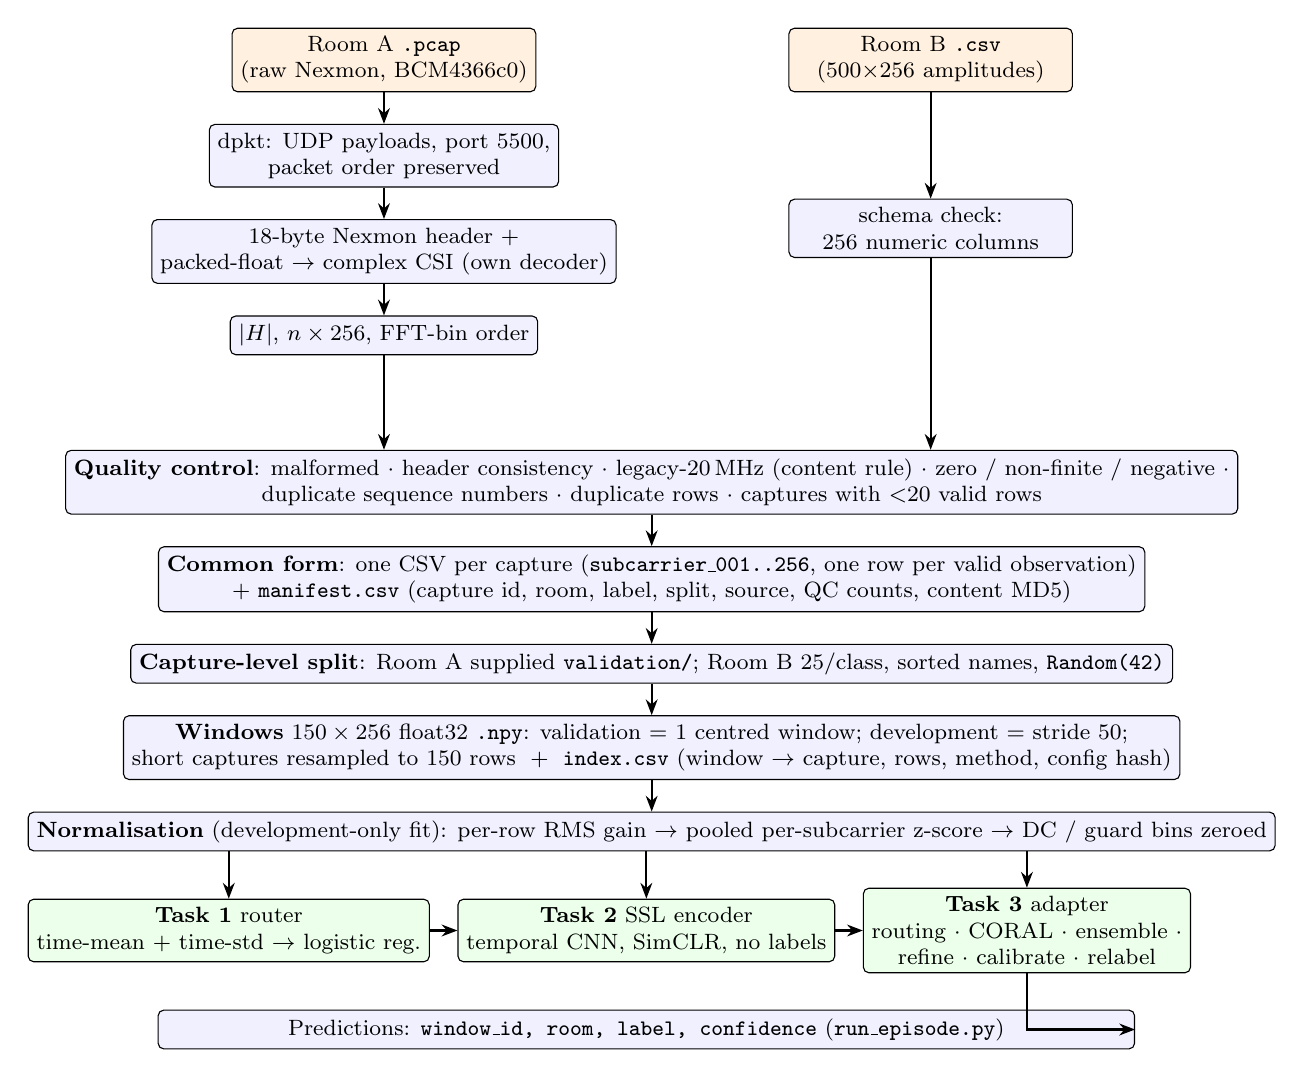
\begin{tikzpicture}[
  node distance=4mm and 6mm,
  box/.style={draw, rounded corners=2pt, fill=blue!6, align=center, font=\footnotesize, minimum width=3.6cm, inner sep=3pt},
  wide/.style={box, minimum width=12.4cm},
  src/.style={box, fill=orange!12},
  task/.style={box, fill=green!8, minimum width=3.9cm},
  arr/.style={-{Stealth[length=2mm]}, thick}]
\node[src] (pcap) {Room A \texttt{.pcap}\\(raw Nexmon, BCM4366c0)};
\node[src, right=3.2cm of pcap] (csv) {Room B \texttt{.csv}\\(500$\times$256 amplitudes)};
\node[box, below=of pcap] (udp) {dpkt: UDP payloads, port 5500,\\packet order preserved};
\node[box, below=of udp] (hdr) {18-byte Nexmon header +\\packed-float $\rightarrow$ complex CSI (own decoder)};
\node[box, below=of hdr] (amp) {$|H|$, $n\times256$, FFT-bin order};
\node[box, below=of csv, yshift=-9.5mm] (schema) {schema check:\\256 numeric columns};
\node[wide, below=12mm of amp, xshift=3.4cm] (qc) {\textbf{Quality control}: malformed $\cdot$ header consistency $\cdot$ legacy-20\,MHz (content rule) $\cdot$ zero / non-finite / negative $\cdot$\\duplicate sequence numbers $\cdot$ duplicate rows $\cdot$ captures with $<$20 valid rows};
\node[wide, below=of qc] (common) {\textbf{Common form}: one CSV per capture (\texttt{subcarrier\_001..256}, one row per valid observation)\\+ \texttt{manifest.csv} (capture id, room, label, split, source, QC counts, content MD5)};
\node[wide, below=of common] (split) {\textbf{Capture-level split}: Room A supplied \texttt{validation/}; Room B 25/class, sorted names, \texttt{Random(42)}};
\node[wide, below=of split] (win) {\textbf{Windows} $150\times256$ float32 \texttt{.npy}: validation = 1 centred window; development = stride 50;\\short captures resampled to 150 rows \;+\; \texttt{index.csv} (window $\rightarrow$ capture, rows, method, config hash)};
\node[wide, below=of win] (norm) {\textbf{Normalisation} (development-only fit): per-row RMS gain $\rightarrow$ pooled per-subcarrier z-score $\rightarrow$ DC / guard bins zeroed};
\node[task, below=6mm of norm.south west, anchor=north west] (t1) {\textbf{Task 1} router\\time-mean + time-std $\rightarrow$ logistic reg.};
\node[task, right=0.35cm of t1] (t2) {\textbf{Task 2} SSL encoder\\temporal CNN, SimCLR, no labels};
\node[task, right=0.35cm of t2] (t3) {\textbf{Task 3} adapter\\routing $\cdot$ CORAL $\cdot$ ensemble $\cdot$\\refine $\cdot$ calibrate $\cdot$ relabel};
\node[wide, below=6mm of t2] (out) {Predictions: \texttt{window\_id, room, label, confidence} (\texttt{run\_episode.py})};
\draw[arr] (pcap) -- (udp); \draw[arr] (udp) -- (hdr); \draw[arr] (hdr) -- (amp);
\draw[arr] (csv) -- (schema);
\draw[arr] (amp.south) -- (amp.south |- qc.north);
\draw[arr] (schema.south) -- (schema.south |- qc.north);
\draw[arr] (qc) -- (common); \draw[arr] (common) -- (split); \draw[arr] (split) -- (win); \draw[arr] (win) -- (norm);
\draw[arr] (norm.south -| t1.north) -- (t1.north);
\draw[arr] (norm.south -| t2.north) -- (t2.north);
\draw[arr] (norm.south -| t3.north) -- (t3.north);
\draw[arr] (t1.east) -- (t2.west);
\draw[arr] (t2.east) -- (t3.west);
\draw[arr] (t3.south) |- (out.east);
\end{tikzpicture}
\caption{Preprocessing and learning pipeline. Room A enters at the packet level and Room B at the amplitude level. After QC both share one code path. The router feeds Task~3's routing; the encoder feeds Task~3's embeddings.}
\label{fig:pipeline}
\end{figure}

\subsection{CSI reconstruction (Room A)}
\texttt{pcap\_reader.py} uses \texttt{dpkt}, a general-purpose pcap parser, only to strip the Ethernet/IP/UDP layers. Everything after the UDP payload is our own code (\texttt{csi\_decode.py}).

\paragraph{Header.} The 18-byte little-endian header holds: magic \texttt{0x1111}, RSSI, frame control, source MAC, sequence number, core/stream, chanspec and chip.

\paragraph{CSI words.} The BCM4366c0 does not export int16 I/Q. Each 32-bit word packs:
\begin{itemize}
  \item the sign of I (bit 29) and an 11-bit I magnitude (bits 18--28);
  \item the sign of Q (bit 17) and an 11-bit Q magnitude (bits 6--16);
  \item a shared 6-bit two's-complement exponent (bits 0--5).
\end{itemize}
We reconstruct $\text{sign}\cdot m\cdot2^{e}$, vectorised over all packets of a capture. Following the public Nexmon format description~\cite{nexmon}, each packet is then rescaled by a power of two so that its largest component occupies 10 bits.

Amplitude is $|H|=\sqrt{I^2+Q^2}$, kept in FFT-bin order, which matches Room~B. The decoded spectra show a zero DC bin, an 11-bin central guard band, smooth frequency-selective fading and visible pilots (Fig.~\ref{fig:qc}). We did not hard-code the null bins: the bins our normalisation detects as near-empty are exactly those the 802.11ac VHT80 layout predicts (DC 0, 1, 255; guard 123--133). This is an independent check that the decoder is correct.

\subsection{Quality control}
Every rule returns a keep-mask and a reason label. Per-capture rejection counts go into the manifest (Table~\ref{tab:qc}).

\begin{table}[H]
\centering\small
\caption{Quality-control rules and rejections.}
\label{tab:qc}
\begin{tabular}{p{5.2cm}rrp{5.4cm}}
\toprule
Rule & Room A & Room B & Rationale\\
\midrule
malformed payload (magic/length) & 2 & n/a & not a 256-subcarrier record\\
header inconsistency & 0 & n/a & a different radio setting is a different observation type\\
legacy-20\,MHz (max sub-band energy $>0.9$) & 165{,}209 & 44{,}425 & sounds only 64 of 256 subcarriers\\
zero / constant / non-finite / negative & 0 & 0 & no information, or invalid\\
duplicate sequence number & 600 & n/a & MAC retransmission of the same frame\\
duplicate consecutive row & 0 & 0 & repeated observation\\
capture with $<20$ valid rows & 7 captures & 0 & no meaningful window\\
\bottomrule
\end{tabular}
\end{table}

\\paragraph{The legacy-20\,MHz rule is the important one.} It removes 71\% of Room~A frames. The rule splits the spectrum into four 20\,MHz sub-bands and rejects a frame if more than 90\% of its energy falls in one of them. On Room~A the statistic is cleanly bimodal (VHT80 $\le0.8$, legacy $\ge0.95$), so the threshold is not sensitive.

We decide on CSI \emph{content}, not on the sequence field, because 47{,}306 legacy frames carry normal sequence numbers. The same rule runs on Room~B (7.4\% of rows), so both rooms pass an identical validity test.

After QC, Room~A has 68{,}210 valid observations (median 59 per capture) and Room~B has 556{,}075. One Room~A validation capture (\texttt{sit201}) keeps only 2 valid frames and is excluded, leaving 149 Room~A validation windows.

\subsection{Common form, splits and provenance}
Both rooms are written as one CSV per capture with columns \texttt{subcarrier\_001..256}. From this point on, the pipeline cannot tell whether a capture began as a pcap or a CSV.

The splits:
\begin{itemize}
  \item \textbf{Room~A validation} is the supplied \texttt{validation/} folder.
  \item \textbf{Room~B validation} takes 25 captures per class. Within each class, candidate names are sorted and drawn with \texttt{random.Random(42).sample}, using a fresh RNG per class. The remaining 1{,}076 captures are development data.
\end{itemize}

The capture is the atomic unit everywhere. A content MD5 hash per capture guards against duplicated recordings crossing the split (none were found). \texttt{index.csv} links every window to its capture, its intermediate CSV, the rows used, the windowing method, and a hash of the configuration that produced it.

\subsection{Windowing and normalisation}
\paragraph{Windowing.}
\begin{itemize}
  \item \textbf{Validation captures} give exactly one centred window, so scoring is capture-level.
  \item \textbf{Development captures} give sliding windows with stride 50. These are augmentation only: $K$ always counts captures.
  \item \textbf{Room~A captures} all have fewer than 150 valid rows (20--118). We \emph{resample} them to 150 rows by linear interpolation, a $\approx$2.5$\times$ uniform time stretch, instead of edge-padding. The length of a padding block would reveal capture length, which is a forbidden metadata cue.
\end{itemize}

\paragraph{Normalisation.}
\begin{enumerate}
  \item Each row is divided by its RMS over the data bins. Autoscale and AGC make the absolute packet level non-physical.
  \item Per-subcarrier z-scores use means and standard deviations fitted on \emph{development windows only}, pooled over both rooms. Pooling means no room label is needed at transform time.
  \item Bins below 5\% of the median development level (DC and guard) are set to zero, so their noise is not amplified.
\end{enumerate}

\subsection{Design rationale}
Table~\ref{tab:rationale} summarises the main decisions and the alternatives we rejected.

\begin{table}[H]
\centering\small
\caption{Key design decisions.}
\label{tab:rationale}
\begin{tabular}{p{3.3cm}p{5.6cm}p{6.2cm}}
\toprule
Decision & Choice & Why / rejected alternative\\
\midrule
CSI decoding & own vectorised 4366c0 packed-float decoder & required by the rules; int16 I/Q decoding gives nonsense spectra\\
Legacy frames & reject on sub-band energy content & sequence \texttt{0xFFFF} misses 47k legacy frames\\
Short captures & linear time resampling & edge padding leaks capture length\\
Validation windows & one centred window per capture & long captures cannot dominate the score\\
Gain & per-row RMS & autoscale/AGC make absolute level meaningless\\
Standardisation & pooled, development-only & no room label needed at transform time; no leakage\\
Null bins & detected from data, zeroed, 256 columns kept & Hint 5: do not silently drop subcarriers\\
Room-specific statistics & at embedding level, chosen by the router & keeps the SSL stage free of room labels\\
Shared SIT/STAND/WALK & target-room clusters named by a motion prior & direct cross-room transfer swaps WALK and SIT; per-class calibration cannot undo a swap\\
\bottomrule
\end{tabular}
\end{table}

%==========================================================================
\section{Task 1: recorded-environment identification}

\paragraph{Method.} For every subcarrier, the router (\texttt{room.py}) takes the time-mean and time-std of the normalised window, giving 512 features. These go through standardisation and an L2-regularised logistic regression ($C=0.05$), fitted on all 8{,}462 development windows. The router sees only the amplitude array.

\paragraph{Results.} It classifies all 274 validation windows correctly (A: 149/149, B: 125/125). Linear probes on SSL, random-encoder and handcrafted features also reach 1.000.

\paragraph{Accuracy vs window length.} For each length $L$, we train on random $L$-row sub-windows of development windows and test on the centred $L$-row sub-window of each validation window (Table~\ref{tab:len}, Fig.~\ref{fig:roomlen}).

\begin{table}[H]
\centering\small
\caption{Room accuracy against window length $L$ (fixed validation capture pool).}
\label{tab:len}
\begin{tabular}{lcccccccc}
\toprule
$L$ & 1 & 2 & 5 & 10 & 25 & 50 & 100 & 150\\
\midrule
all windows & 0.978 & 1.000 & 0.996 & 0.996 & 1.000 & 1.000 & 1.000 & 1.000\\
Room A & 0.960 & 1.000 & 0.993 & 0.993 & 1.000 & 1.000 & 1.000 & 1.000\\
Room B & 1.000 & 1.000 & 1.000 & 1.000 & 1.000 & 1.000 & 1.000 & 1.000\\
\bottomrule
\end{tabular}
\end{table}

\paragraph{Interpretation.} The rooms differ in much more than geometry:
\begin{itemize}
  \item the static multipath profile, which is the intended signal;
  \item the guard-band noise floor;
  \item per-row variability (Table~\ref{tab:lag});
  \item smoothness, because Room~A windows are resampled.
\end{itemize}
The fingerprint therefore identifies the \emph{recorded environment and session}. It does not show that a model could recognise a third room.

%==========================================================================
\section{Task 2: learning without labels}

\paragraph{Encoder.} A 1-D temporal CNN over the $(T,256)$ window:
\begin{itemize}
  \item a $1\times1$ ``spectral'' convolution from 256 to 128 channels;
  \item four temporal blocks (kernels 7/5/5/3, strides 1/2/2/2);
  \item mean and standard-deviation pooling over time, followed by a linear layer producing a 128-d embedding.
\end{itemize}

\paragraph{Objective.} SimCLR NT-Xent~\cite{simclr} ($\tau=0.2$) with a 2-layer projection head.
\begin{itemize}
  \item Batches are drawn per \emph{capture}. Capture identity is provenance, not a label.
  \item The two views of a capture are two of its windows.
  \item Augmentations: random crop (96--150 rows), global gain $\times[0.8,1.25]$, a smooth per-subcarrier gain tilt, Gaussian noise, subcarrier-band masking, and time masking.
  \item Time reversal is excluded because SIT-DOWN and STAND-UP are near time-reversals of each other.
  \item Training: 60 epochs, AdamW, one-cycle learning rate. No activity or room labels are used.
\end{itemize}
The loss falls from 4.87 to 1.80 (Fig.~\ref{fig:ssl}).

\paragraph{Evaluation.} The encoder is frozen. A class-balanced logistic regression is fitted on labelled development embeddings and scored on validation windows. We compare against two baselines:
\begin{itemize}
  \item the same CNN with random weights;
  \item handcrafted features: per-band temporal mean, std, mean $|\Delta|$ and range over 32 subcarrier bands, four Doppler-band energies, and the dominant-PC variance ratio.
\end{itemize}

\begin{table}[H]
\centering\small
\caption{Linear-probe results on validation windows (macro-F1 / balanced accuracy). ``Shared'' trains on one room's SIT/STAND/WALK and tests on the other room.}
\label{tab:ssl}
\begin{tabular}{lccccc}
\toprule
Representation & Room A (6) & Room B (5) & Joint (8) & Shared A$\to$B & Shared B$\to$A\\
\midrule
\textbf{SSL encoder} & \textbf{0.932} / 0.933 & \textbf{0.992} / 0.992 & \textbf{0.946} / 0.957 & 0.235 / 0.213 & 0.175 / 0.280\\
random weights & 0.891 / 0.892 & 0.790 / 0.792 & 0.738 / 0.771 & 0.167 / 0.333 & 0.168 / 0.333\\
handcrafted & 0.932 / 0.933 & 0.992 / 0.992 & 0.909 / 0.924 & 0.167 / 0.333 & 0.168 / 0.333\\
\bottomrule
\end{tabular}
\end{table}

\paragraph{Findings.}
\begin{itemize}
  \item Self-supervision beats random weights in every within-room setting: +0.20 on Room~B and +0.21 on the joint task. It matches or beats the handcrafted features.
  \item The UMAP plot (Fig.~\ref{fig:umap}) shows rooms separating completely. Within a room, the SSL embedding forms compact activity clusters, while the random encoder mixes them.
  \item The ``shared'' columns stay at chance for every representation. This is the first sign of the Task~3 transfer problem.
\end{itemize}

%==========================================================================
\section{Task 3: cross-room few-label adaptation}

\subsection{Method}
An episode is defined by a target room $T$, a value of $K$, and a support seed (0--4).
\begin{enumerate}
  \item \textbf{Support.} For each $T$-exclusive activity, draw $K$ distinct $T$-development captures. All of their windows are used, but $K$ counts captures.
  \item \textbf{Routing.} The Task~1 router predicts each validation window's room. The routed room selects (a) the alignment statistics and (b) the label space: a window routed to room $R$ can only receive $R$'s activities.
  \item \textbf{Alignment.} SSL embeddings are whitened with the mean and shrunk full covariance of their room's \emph{unlabelled} development embeddings (CORAL-style~\cite{coral}, a feature-level analogue of AdaBN~\cite{adabn}).
  \item \textbf{Ensemble classifier.} The class probabilities of two heads are averaged:
  \begin{itemize}
    \item a cosine nearest-prototype head~\cite{protonet} (temperature 0.1), averaging per-capture means;
    \item a class-balanced logistic regression.
  \end{itemize}
  Shared classes are learned from all labelled source-development windows; exclusive classes from the $K$ support captures.
  \item \textbf{Refinement.} Soft $k$-means over the target's unlabelled development windows (never validation), with a Sinkhorn~\cite{sinkhorn} balancing step and the support means as anchors.
  \item \textbf{Calibration.} Per-class logit offsets are fitted so that predictions on unlabelled target-development windows are class-balanced (log-domain column scaling). The offsets are then applied to validation windows.
  \item \textbf{Shared-activity relabelling} (\texttt{fewshot.relabel\_shared}). Steps 1--6 decide well \emph{whether} a window is a shared activity, but transferring \emph{which} one from the source room fails (Section~\ref{sec:disc}). The shared label is therefore taken from the target room itself:
  \begin{itemize}
    \item The classifier labels the target room's unlabelled development windows. Those it calls SIT, STAND or WALK are clustered with $k$-means on standardised handcrafted features concatenated with the aligned SSL embedding.
    \item Each cluster is named by the rank of its median \textbf{slow-motion score} under the prior WALK $>$ STAND $>$ SIT. The lowest third of clusters become SIT, the middle third STAND, and the top third WALK. The score is the temporal std of band-averaged amplitudes after a 9-row moving average, which removes Room~B's row-to-row ripple (\texttt{features.motion\_features}).
    \item A validation window the classifier calls shared takes the name of its nearest cluster. This is repeated for $k=9,12,15$ and the three labels are combined by majority vote. Target-exclusive predictions are unchanged.
  \end{itemize}
  The prior is physical, not learned: walking moves the whole body, and standing has more postural sway than sitting. It holds in both rooms' development data (median score, Room~A: WALK 0.259, STAND 0.048, SIT 0.019; Room~B: WALK 0.220, STAND 0.203, SIT 0.196, EMPTY 0.141).
\end{enumerate}
No target SIT/STAND/WALK labels and no validation data are used at any step.

\subsection{Results}
\begin{table}[H]
\centering\small
\caption{Main method, mean $\pm$ std over 5 support seeds (validation). B$\to$A means target room A.}
\label{tab:t3}
\begin{tabular}{llcccc}
\toprule
Metric & Target & $K=1$ & $K=5$ & $K=10$ & $K=20$\\
\midrule
primary macro-F1 & A & 0.402$\pm$0.056 & 0.546$\pm$0.031 & 0.658$\pm$0.050 & 0.740$\pm$0.020\\
 & B & 0.333$\pm$0.038 & 0.636$\pm$0.137 & 0.632$\pm$0.061 & 0.725$\pm$0.029\\
target-exclusive macro-F1 & A & 0.395$\pm$0.068 & 0.570$\pm$0.031 & 0.711$\pm$0.029 & 0.793$\pm$0.035\\
 & B & 0.247$\pm$0.045 & 0.669$\pm$0.126 & 0.788$\pm$0.069 & 0.860$\pm$0.040\\
shared macro-F1 & A & 0.408$\pm$0.060 & 0.523$\pm$0.066 & 0.604$\pm$0.086 & 0.688$\pm$0.055\\
 & B & 0.391$\pm$0.044 & 0.614$\pm$0.149 & 0.528$\pm$0.109 & 0.636$\pm$0.066\\
balanced accuracy & A & 0.403$\pm$0.055 & 0.544$\pm$0.041 & 0.657$\pm$0.049 & 0.736$\pm$0.026\\
 & B & 0.338$\pm$0.050 & 0.629$\pm$0.144 & 0.622$\pm$0.058 & 0.710$\pm$0.032\\
\bottomrule
\end{tabular}
\end{table}

Target-exclusive macro-F1 is identical to the method without relabelling, because relabelling only changes windows predicted as shared. Shared F1 still grows with $K$, although $K$ labels only exclusive activities: better support makes the shared-vs-exclusive decision cleaner, so the clusters contain fewer exclusive windows.

\begin{figure}[H]
\centering
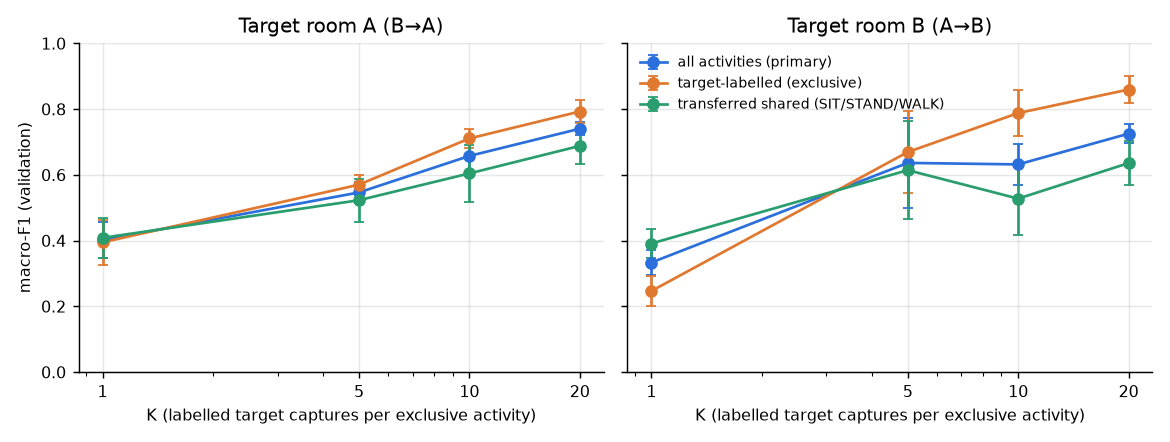
\includegraphics[width=0.9\linewidth]{fig_label_efficiency.png}
\caption{Label-efficiency curve: macro-F1 against $K$ for each target room, with separate curves for target-labelled (exclusive) and transferred shared activities.}
\label{fig:le}
\end{figure}

\paragraph{Routing contribution.} Predicted-room routing equals oracle routing because the router is 100\% accurate on validation (Table~\ref{tab:route}, Fig.~\ref{fig:route}).

Removing routing means pooled alignment statistics and the union label space. Source-room activities (for example EMPTY/LYING for target~A) then steal target windows. At $K=20$ this costs 0.20 (target~A) and 0.34 (target~B) macro-F1. Target~A at $K=1$ is the one cell where routing does not help (0.426 vs 0.402).

\begin{table}[H]
\centering\small
\caption{Routing contribution (primary macro-F1).}
\label{tab:route}
\begin{tabular}{llcccc}
\toprule
Target & Routing & $K=1$ & $K=5$ & $K=10$ & $K=20$\\
\midrule
A & predicted room & 0.402 & 0.546 & 0.658 & 0.740\\
A & oracle room & 0.402 & 0.546 & 0.658 & 0.740\\
A & no routing & 0.426 & 0.434 & 0.509 & 0.543\\
B & predicted room & 0.333 & 0.636 & 0.632 & 0.725\\
B & oracle room & 0.333 & 0.636 & 0.632 & 0.725\\
B & no routing & 0.276 & 0.383 & 0.380 & 0.383\\
\bottomrule
\end{tabular}
\end{table}

\paragraph{Ablations.} Unless a row says otherwise, every variant uses the ensemble head, refinement, calibration and relabelling (Table~\ref{tab:abl}, Fig.~\ref{fig:abl}).

\begin{table}[H]
\centering\footnotesize\setlength{\tabcolsep}{4pt}
\caption{Ablations (primary macro-F1, mean over 5 seeds).}
\label{tab:abl}
\begin{tabular}{@{}l*{9}{c}@{}}
\toprule
Variant & A1 & A5 & A10 & A20 & B1 & B5 & B10 & B20 & avg\\
\midrule
\textbf{main} & 0.402 & 0.546 & 0.658 & 0.740 & 0.333 & 0.636 & 0.632 & 0.725 & \textbf{0.584}\\
no relabelling (second main) & 0.266 & 0.337 & 0.397 & 0.464 & 0.213 & 0.379 & 0.435 & 0.434 & 0.366\\
prototype-only (first main) & 0.258 & 0.300 & 0.376 & 0.447 & 0.235 & 0.378 & 0.395 & 0.422 & 0.352\\
relabel on handcrafted only & 0.379 & 0.541 & 0.613 & 0.672 & 0.322 & 0.588 & 0.609 & 0.711 & 0.555\\
relabel on motion features & 0.428 & 0.577 & 0.678 & 0.738 & 0.265 & 0.476 & 0.530 & 0.562 & 0.532\\
no calibration & 0.422 & 0.548 & 0.661 & 0.709 & 0.356 & 0.591 & 0.614 & 0.747 & 0.581\\
no refinement & 0.401 & 0.575 & 0.682 & 0.708 & 0.331 & 0.480 & 0.689 & 0.713 & 0.572\\
diagonal alignment & 0.365 & 0.512 & 0.609 & 0.585 & 0.330 & 0.525 & 0.548 & 0.591 & 0.508\\
logistic regression only$^\dagger$ & 0.249 & 0.385 & 0.469 & 0.484 & 0.147 & 0.325 & 0.384 & 0.417 & 0.358\\
random-weight encoder & 0.388 & 0.534 & 0.568 & 0.584 & 0.353 & 0.461 & 0.479 & 0.545 & 0.489\\
handcrafted features & 0.321 & 0.439 & 0.487 & 0.594 & 0.293 & 0.524 & 0.581 & 0.616 & 0.482\\
SSL, static profile removed & 0.217 & 0.304 & 0.338 & 0.374 & 0.322 & 0.519 & 0.561 & 0.573 & 0.401\\
\bottomrule
\multicolumn{10}{l}{\footnotesize $^\dagger$ no refinement, calibration or relabelling.}
\end{tabular}
\end{table}

\begin{itemize}
  \item \textbf{Shared-activity relabelling is the largest gain:} the 8-cell average rises from 0.366 to 0.584, with a gain in every cell. Shared macro-F1 rises from 0.08--0.20 to 0.39--0.69.
  \item \textbf{Relabelling feature space.} The 3 motion features alone are best for target~A, where WALK is $13\times$ more mobile than SIT. They are worst for target~B (shared F1 0.28--0.36), where the motion gaps are a few percent. Handcrafted features plus the aligned SSL embedding are the best single choice for both rooms (0.584 vs 0.555 for handcrafted only). We use one setting for both directions, not a per-room choice.
  \item \textbf{Routing} helps in 7 of 8 cells, by up to 0.34.
  \item \textbf{SSL pretraining} is now the best representation for both targets at $K\ge10$: for example 0.725 vs 0.545 (random) and 0.616 (handcrafted) for target~B at $K=20$.
  \item \textbf{CORAL} beats diagonal alignment in all 8 cells.
  \item \textbf{Refinement and calibration} are within noise on average (0.572 and 0.581 without them, vs 0.584). Refinement gives the largest single-cell gain (+0.16, target~B, $K=5$).
  \item \textbf{Removing the static profile} before the encoder is worse in every cell.
\end{itemize}

\paragraph{Confusion matrices at $K=5$} (support seed 0; Fig.~\ref{fig:cm}, Table~\ref{tab:cm}).
\begin{itemize}
  \item \textbf{Before relabelling:} target WALK was predicted mostly as SIT (A: 18/25, B: 14/25), and WALK F1 was 0.00 in both rooms.
  \item \textbf{After relabelling:} target WALK $\to$ SIT falls to 0/25 (A) and 5/25 (B). WALK F1 is 0.79 in both rooms, and SIT F1 is 0.67 (A) and 0.71 (B; recall 25/25).
  \item \textbf{Remaining errors:} target-A STAND is mostly sent to exclusive classes (FALL 9, SIT-DOWN 5, STAND-UP 3 of 25), and target-B LYING goes to STAND/WALK (11/25).
\end{itemize}

\begin{table}[H]
\centering\small
\caption{Per-activity precision / recall / F1 at $K=5$ (seed 0).}
\label{tab:cm}
\begin{tabular}{lccc@{\hspace{1.2cm}}lccc}
\toprule
Target A & P & R & F1 & Target B & P & R & F1\\
\midrule
SIT & 0.56 & 0.83 & 0.67 & SIT & 0.56 & 1.00 & 0.71\\
STAND & 0.42 & 0.20 & 0.27 & STAND & 0.68 & 0.60 & 0.64\\
WALK & 0.83 & 0.76 & 0.79 & WALK & 0.83 & 0.76 & 0.79\\
SIT-DOWN & 0.44 & 0.44 & 0.44 & EMPTY & 1.00 & 0.84 & 0.91\\
STAND-UP & 0.73 & 0.76 & 0.75 & LYING & 0.79 & 0.44 & 0.56\\
FALL & 0.56 & 0.60 & 0.58 & & & & \\
\bottomrule
\end{tabular}
\end{table}

%==========================================================================
\section{Discussion and limitations}\label{sec:disc}

\paragraph{Why shared activities do not transfer directly.} Within a room, activities are easy: probes reach 0.93--0.99 macro-F1. Across rooms, SIT/STAND/WALK transferred from the source room stay at or below chance under every representation and classifier we tried, and the errors are \emph{systematic}. This is why the main method relabels them from the target room instead (step~7). We see three causes.
\begin{enumerate}
  \item \textbf{The archives are different measurements.}
  \begin{itemize}
    \item Room~A frames are smooth in time, and WALK has 5--10$\times$ the temporal variation of SIT.
    \item Room~B rows are independent snapshots (Table~\ref{tab:lag}), and its most variable classes are SIT and STAND.
    \item After alignment, ``high variation'' therefore points to WALK in~A but to SIT/STAND in~B, which reproduces the observed swap.
  \end{itemize}
  \item \textbf{Activity--location confound.} Room~A activities were recorded in different spatial zones, so the static profile partly encodes \emph{where} the person was.
  \item \textbf{Session confound.} Alignment removes first- and second-order room differences, but not class-conditional ones.
\end{enumerate}

\paragraph{A swap is not a collapse.} Calibration balances the predicted class frequencies. That fixes a model that sends everything to one class. Here, however, the target clusters exist and are attached to the wrong source labels, and rebalancing counts cannot un-swap them.

\paragraph{Why relabelling works.} A weak slow-time signal survives in Room~B. After a 9-row moving average, the order WALK $>$ STAND $>$ SIT $>$ EMPTY holds as in Room~A, but with gaps of a few percent instead of an order of magnitude. That is too weak to transfer a classifier, but enough to \emph{name} clusters, and the clusters themselves come from within-room structure, where the classes separate well.

\paragraph{Limitations.}
\begin{itemize}
  \item Room~A windows are time-resampled.
  \item The benchmark is capture-disjoint, not subject-disjoint, and covers only two environments.
  \item Validation results guided several design choices (CORAL, refinement, the ensemble head, calibration, the relabelling feature space and cluster counts), so they are not unseen-test estimates. The motion prior was checked on the development labels of both rooms before use. That is a design decision informed by target-room shared labels, although no such label fits or names any cluster.
  \item Calibration assumes roughly balanced activity frequencies in the target room.
  \item Relabelling depends on the prior WALK $>$ STAND $>$ SIT and on the clusters splitting into motion tertiles. In Room~B the gaps are small, so cluster naming is the fragile step. It also needs unlabelled target-room recordings of each shared activity.
  \item The original paper's random 80/20 results answer a different question and are not comparable.
\end{itemize}

\paragraph{Future work.} Choosing the cluster count and the relabelling feature space per room without validation (for example by a silhouette criterion); combining the motion prior with the \emph{relational} structure of target clusters and source prototypes; complex-CSI recordings in both rooms, so that phase features can be compared.

%==========================================================================
\section{Implementation and reproducibility}

\begin{itemize}
  \item \textbf{Environment:} Python~3.11 with pinned versions in \texttt{requirements.txt} (CPU-only PyTorch).
  \item \textbf{Full run:} \texttt{python run\_all.py} runs inspect $\to$ dataset $\to$ ssl $\to$ task1 $\to$ task2 $\to$ task3 $\to$ figures, about 70\,min on a 10-core laptop CPU (60\,min of it is SSL training).
  \item \textbf{Episodes:} \texttt{run\_episode.py --episode DIR} sends arbitrary \texttt{.pcap}, 256-column \texttt{.csv} or $(150,256)$ \texttt{.npy} queries, plus optional labelled \texttt{support/}, through the same decode $\to$ QC $\to$ window $\to$ normalise $\to$ route $\to$ embed $\to$ classify path. It writes \texttt{window\_id, room, label, confidence}.
  \item \textbf{Outputs:} every Task~3 episode is logged as \texttt{experiment, target\_room, K, metric, value, seed} in \texttt{results/task3\_results.csv}.
  \item \textbf{Code layout:}
  \begin{itemize}
    \item \texttt{pcap\_reader.py}, \texttt{csi\_decode.py}, \texttt{amplitude.py} --- ingestion;
    \item \texttt{cleaning.py}, \texttt{ingest.py}, \texttt{splits.py} --- QC, common form and splits;
    \item \texttt{windowing.py}, \texttt{dataset.py}, \texttt{normalization.py} --- model input;
    \item \texttt{features.py}, \texttt{models.py}, \texttt{ssl.py}, \texttt{room.py}, \texttt{fewshot.py} --- learning.
  \end{itemize}
\end{itemize}

%==========================================================================
\section{Required figures}

\begin{figure}[H]
\centering
\includegraphics[width=0.95\linewidth]{fig_qc_examples.png}
\caption{QC examples: decoded Room A spectrum (valid VHT80 frames vs rejected legacy 20\,MHz frames), a Room A valid-frame spectrogram, and a raw Room B window.}
\label{fig:qc}
\end{figure}

\begin{figure}[H]
\centering
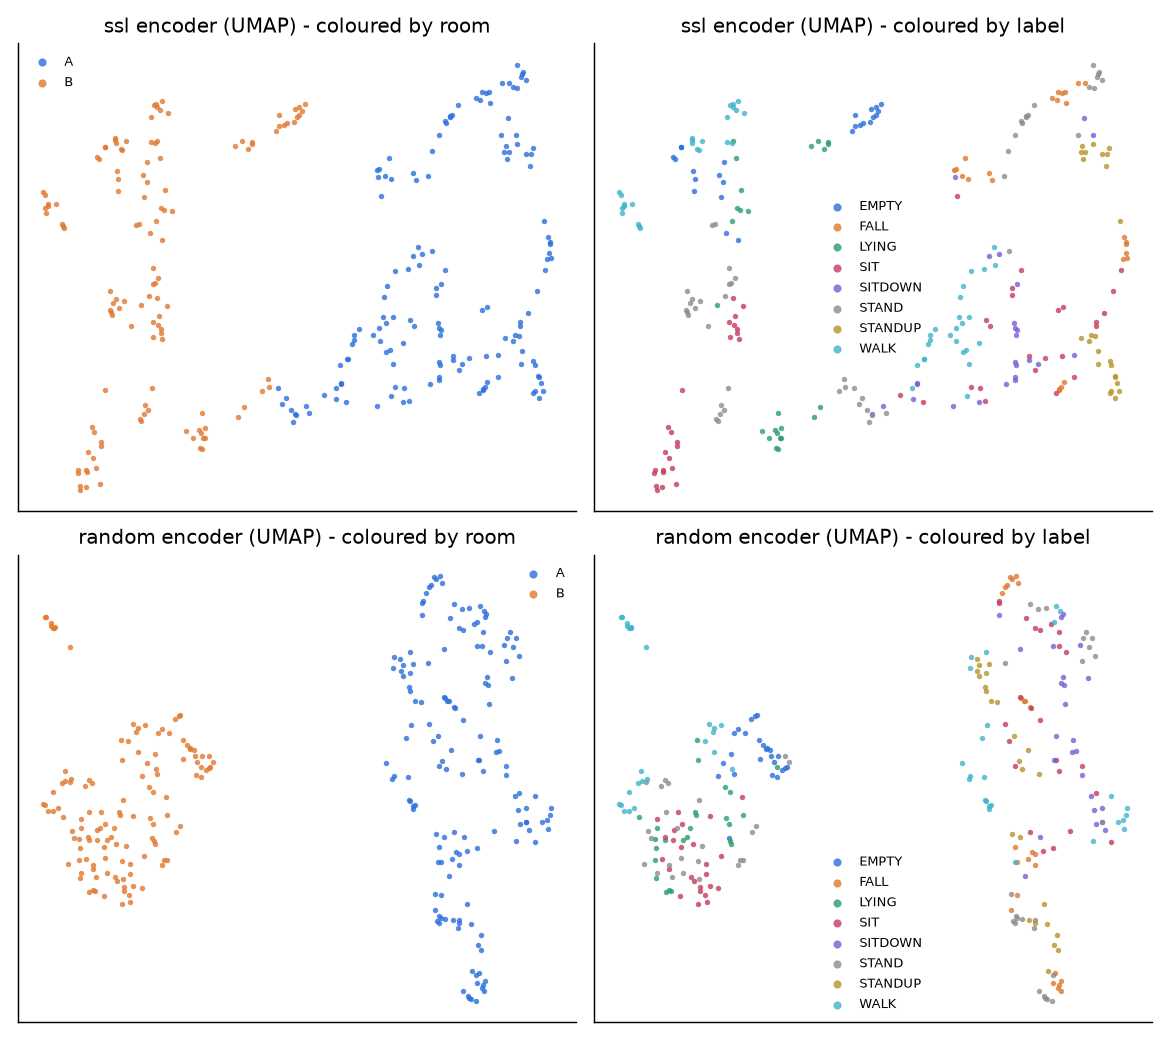
\includegraphics[width=0.95\linewidth]{fig_embedding_2d.png}
\caption{Encoder diagnosis: UMAP of validation embeddings, coloured by room and by activity (SSL vs random weights). Qualitative only.}
\label{fig:umap}
\end{figure}

\begin{figure}[H]
\centering
\begin{minipage}{0.48\linewidth}\centering
\includegraphics[width=\linewidth]{fig_room_vs_length.png}
\caption{Environment fingerprint: room accuracy against window length.}
\label{fig:roomlen}
\end{minipage}\hfill
\begin{minipage}{0.48\linewidth}\centering
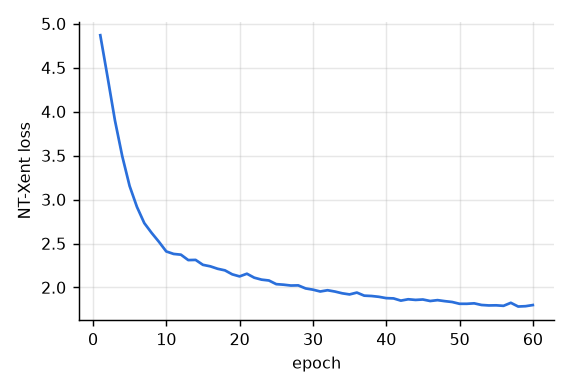
\includegraphics[width=\linewidth]{fig_ssl_loss.png}
\caption{SSL training loss.}
\label{fig:ssl}
\end{minipage}
\end{figure}

\begin{figure}[H]
\centering
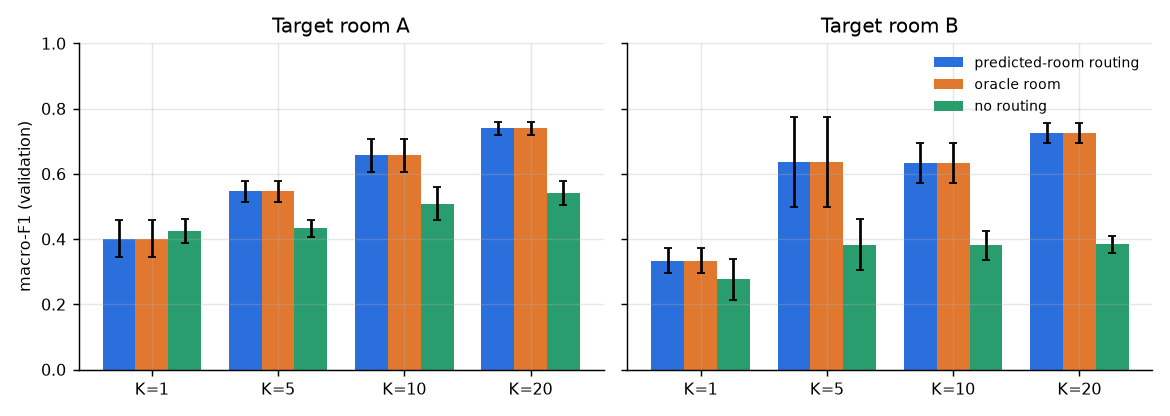
\includegraphics[width=0.9\linewidth]{fig_routing.png}
\caption{Routing contribution: predicted-room routing vs oracle room vs no routing.}
\label{fig:route}
\end{figure}

\begin{figure}[H]
\centering
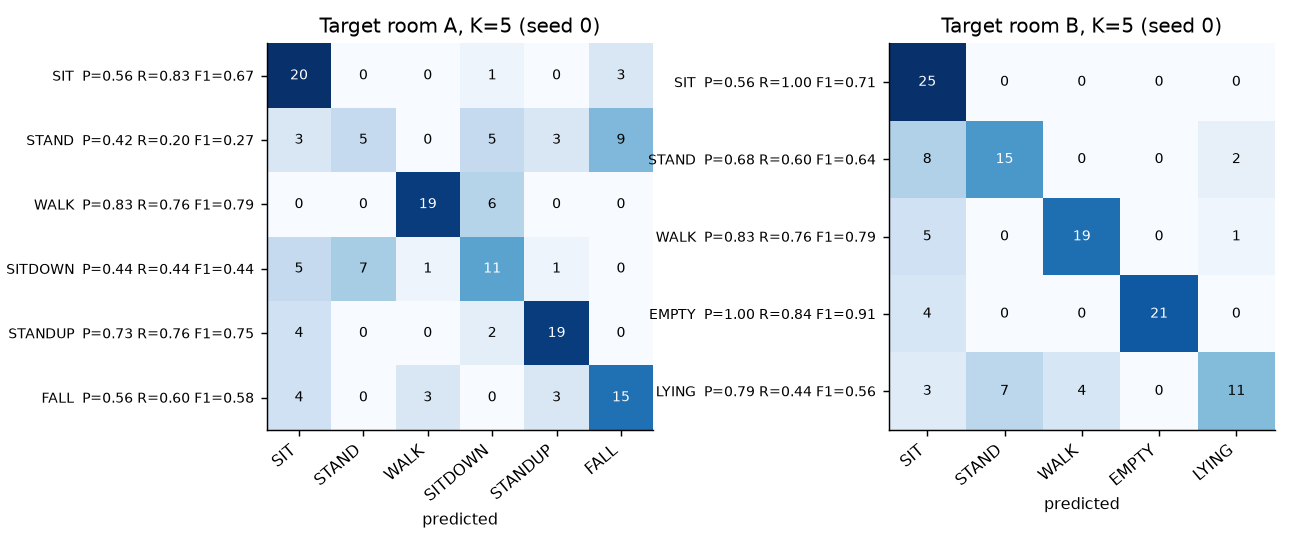
\includegraphics[width=0.95\linewidth]{fig_confusion_K5.png}
\caption{Confusion matrices at $K=5$ (seed 0), one per target room, with per-activity precision, recall and F1.}
\label{fig:cm}
\end{figure}

\begin{figure}[H]
\centering
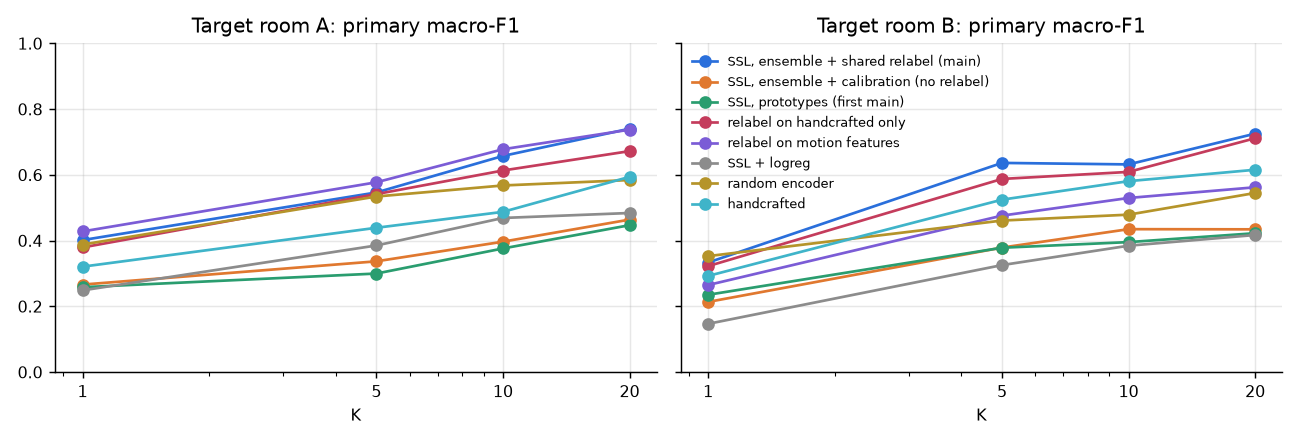
\includegraphics[width=0.9\linewidth]{fig_ablation.png}
\caption{Ablation of relabelling, representation and head (primary macro-F1).}
\label{fig:abl}
\end{figure}

%==========================================================================
\section{Pipeline independence, contribution and AI-use disclosure}

\paragraph{Pipeline independence.} No source-author code, MATLAB, notebooks, processed \texttt{.mat} files or result files were used or opened.
\begin{itemize}
  \item The Drive folder also contains \texttt{Experiment-2.zip} and \texttt{Experiment-3.zip}, which bundle the authors' code, results and LSTM notebook.
  \item A first version of our download script fetched both archives. We listed their file names and extracted only the two ReadMe PDFs plus one data pcap that had failed to download. The archives were then deleted without opening the code, results or notebook. The download script now skips them.
  \item A later local copy of the data also contained the authors' \texttt{matlab code} and \texttt{Results} folders and the LSTM notebook. These were deleted before any processing, and the pipeline never reads them. \todo{Team: confirm no member opened them.}
\end{itemize}
The 4366c0 decoder follows the public Nexmon format description and is our own implementation. \texttt{dpkt} is used only for generic packet parsing.

\paragraph{Contribution statement.} \todo{To be completed by the team: who did ingestion and decoding, QC and windowing, SSL, few-shot adaptation, evaluation, and the report.}

\paragraph{AI-use disclosure.} This project was developed with substantial help from an AI coding assistant (Claude, Anthropic, used through Claude Code). The assistant was used for:
\begin{itemize}
  \item data inspection;
  \item implementing the pipeline modules;
  \item running the experiments, including the Room~B lag analysis and the Task~3 ensemble, calibration and relabelling variants;
  \item drafting this report.
\end{itemize}
\todo{The team must review, understand and be able to explain every stage, and should edit this paragraph to describe their actual use, as required by the course AI-use rules.}

%==========================================================================
\begin{thebibliography}{9}\small
\bibitem{dataport} IEEE DataPort, CSI Human Activity dataset. \url{https://ieee-dataport.org/open-access/csi-human-activity}
\bibitem{schafer} J.~Sch\"afer et al., ``Human Activity Recognition Using CSI Information with Nexmon,'' \emph{Applied Sciences} 11(19):8860, 2021.
\bibitem{nexmon} F.~Gringoli, M.~Schulz, J.~Link, M.~Hollick, ``Free Your CSI: A Channel State Information Extraction Platform for Modern Wi-Fi Chipsets,'' WiNTECH 2019.
\bibitem{simclr} T.~Chen et al., ``A Simple Framework for Contrastive Learning of Visual Representations,'' ICML 2020.
\bibitem{protonet} J.~Snell, K.~Swersky, R.~Zemel, ``Prototypical Networks for Few-shot Learning,'' NeurIPS 2017.
\bibitem{adabn} Y.~Li et al., ``Revisiting Batch Normalization for Practical Domain Adaptation,'' ICLR-W 2017.
\bibitem{coral} B.~Sun, K.~Saenko, ``Deep CORAL: Correlation Alignment for Deep Domain Adaptation,'' ECCV-W 2016.
\bibitem{sinkhorn} M.~Cuturi, ``Sinkhorn Distances: Lightspeed Computation of Optimal Transport,'' NeurIPS 2013.
\end{thebibliography}

\end{document}
